

\chapter{Sprint 1}
\label{Sprint0}
\lhead{Chapter 7. \emph{Sprint 1}}

\section{Goal(s)}

This sprint's goal was the completition of an initial prototype of the system whose functionality
had to be demonstrated to the customer; this corresponded to project milestone M1.
The purpose of such prototype was to act as a proof-of-concept and give the customer
a chance to express some feedback upon which we hoped to start a discussion
on possible improvements and new features.

Additional goals were the completion of project's planning and documents such as:
\begin{enumerate}[a)]
\item system requirements (both functional and non-functional)
\item report's table of contents
\item concrete work plan
\item risk analysis
\item test plan
\end{enumerate}

\section{Planning}

We planned to begin with an initial design and implementation of every part of the system which included:
\begin{enumerate}
\item the frontend, implementing the graphical user interface
\item the backend, implementing the logic of the API
\item the database, implementing persistency
\item the Android application to measure heart rate.
\end{enumerate}
During the first week development was to be done parallel to additional studies and documentation.
The second week we planned to work exclusively on development in view of the impending milestone.

\section{Duration}
The duration of the sprint was the following:
\begin{itemize}
\item Start: September, 9th
\item Milestone M1 (first system prototype): September, 20th
\item End: September, 22nd
\end{itemize}

\begin{figure}[H]
\centering
\includegraphics[scale=0.60]{../Figures/burndownSprint1.png}
\caption{Burndown chart Sprint 0}
\label{figure:burndownsprint0}
\end{figure}

\section{Backlog}

See below the sprint backlog.
\begin{itemize}
	\item \textbf{M1 First system prototype}
		Demonstrated to the customer on September, 20th.
		The demonstration was attended by the customer and two team members.
		The third team member participated remotely via Skype.
	\item \textbf{Project management}\newline
		This included:
		\begin{itemize}
			\item \textbf{Weekly startup meeting}: 
			\item \textbf{Meeting notes}:
				taking notes during meetings, reviewing of the notes.
			\item \textbf{Status reports}:
				for both week 37 and 38
			\item \textbf{Risk analysis}:
				updated on a weekly basis, so twice per sprint.
				The risk analisys was submitted to the supervisor and the customer.
			\item \textbf{Planning for the next iteration}:
				the project manager prepared a plan for the next iteration
				which would be illustrated and agreed upon on next iteration's startup meeting.
		\end{itemize}
	\item \textbf{Weekly meetings}
		includes meetings with both the customer and the supervisor.
		The meeting with the customer was held on Skype.
	\item \textbf{Additional pre-studies}
		Continued studies on relevant technlogies such as:
	\begin{itemize}
		\item \textbf{HealthVault}: Microsoft's online health platform.
		\item \textbf{Apache Camel}: a routing engine for enterprise integration patterns.
		\item \textbf{Javascript libraries for charts}: to be used in the frontend.
	\end{itemize}
	\item \textbf{System development}
		Initial design and implementation. This accounted for:
	\begin{itemize}
		\item \textbf{Backend development}:
			Development of Spring controllers for API endpoints. Database (DAO) coding to
			implement data persistence.
		\item \textbf{Frontend development}:
			Coding of the frontend. This included setting up an HTML page which used
			AJAX to perform API calls and JS to show the data retrieved using a bar chart.
		\item \textbf{Deployment}:
			Deployment of both backend and frontend using a servlet container (Tomcat).
	\end{itemize}
	\item \textbf{Heart rate application}:
		basic implementation of the Heart rate application. The application should be able to acquire
		the user's heart reate and send perform an API call to store the data on the backend.
	\item \textbf{Database development}:
		choose a suitable database to use for implementing persistency on the backend.
		Deploy the database and create a table for the heart rate.
	\item \textbf{Testing}:
		Perform unit and integration testing for the heart rate application and the backend.
\end{itemize}


%% i actually dont think having a table for this is a good idea. tables can't have much information
%% also it would require a lot of tweaking to get the estimated/actual times to look reasonable.
%% maybe a textual description would be better so we can omit some details in favor of others.
\iffalse
\begin{table}
\begin{tabular}{ | l | l | l | l | }
 \hline
  Story ID & Description & Size & Assignee \\
  \hline\noalign{\smallskip}\noalign{\smallskip}\hline
  33 & Project Management			& 8	& Emanuele  \\
  12 & M1 First System prototype	& 0 & All		\\
  45 & Weekly meetings (week 37)	& 6 & All		\\
  42 & Additional pre-studies		& 5 & Emanuele	\\
  \hline
\end{tabular}
\caption{}
\label{}
\end{table}
\fi

\section{Results and feedback}

Around the end of this sprint, on September 20th, we demonstrated a prototype of system to
the client which included: a) the frontend, b) the backend, c) an Android application to measure
heart rate using the phone's camera.

The backend supported web API calls for storing and retrieving heart rate measurements.
Both the Android application and the frontend used these API calls for sending and retrieving
such measurements respectively.
The measurements were ultimately shown to the user on a webpage (the frontend) using a bar chart.
We opted for MySQL as database to implement persistency on the backend due to the familiaritywe had with it.
We deployed it on the server machine and added a first table so that we could test the web API.
%functionality of the backend.
The customer was pleased with the results, stating that they were above his expectations.
We discussed about which features he would like to see implemented next in the product
and we agreed to prioritise interoperability with HealthVault instead of Withings.
The reason behind this decision was the fact that interoperability with HealthVault would have
enabled the product to use third-party devices supported by HealthVault to gather health data.
Since the number of devices supported by HealthVault is substantial, this was deemed a
desiderable feature for the product.
The customer asked if the amounts of resources we had at disposal to actually implement
such interoperability was sufficient and inquired about the general viability of such approach.
We expressed our confidence about its feasibility and that the resources at hand were sufficient.
Nevertheless, we set a deadline (10 days) to assess such feasibility in order not to delay
the general progress of the product.

\textbf{Notes}: by the end of the sprint one team member had found a job and moved permanently to Oslo.
He expressed his continued committment to the project and told the other members that he would continue
to contribute to the project remotely.

\section{Evaluation}

The sprint was successful as we managed to achieve the main goal of the sprint (Milestone M1).
We were pleased by the positive feedback received from the customer and felt motivated to
keep up the good work. Furthermore, having proactively partecipated in the improvement/proposal
of product requirements together with the customer made the whole team look forward to implement these new
features and improve the product. Although we didn't manage write anything in the report we still had enough
time ahead to make up for it so we consider that a minor issue.
Development times for the Android application were dramatically reduced thanks to the functionality
offered by android-heart-rate-monitor (described in section \ref{subsec:hr}).

\begin{figure}[h]
\centering
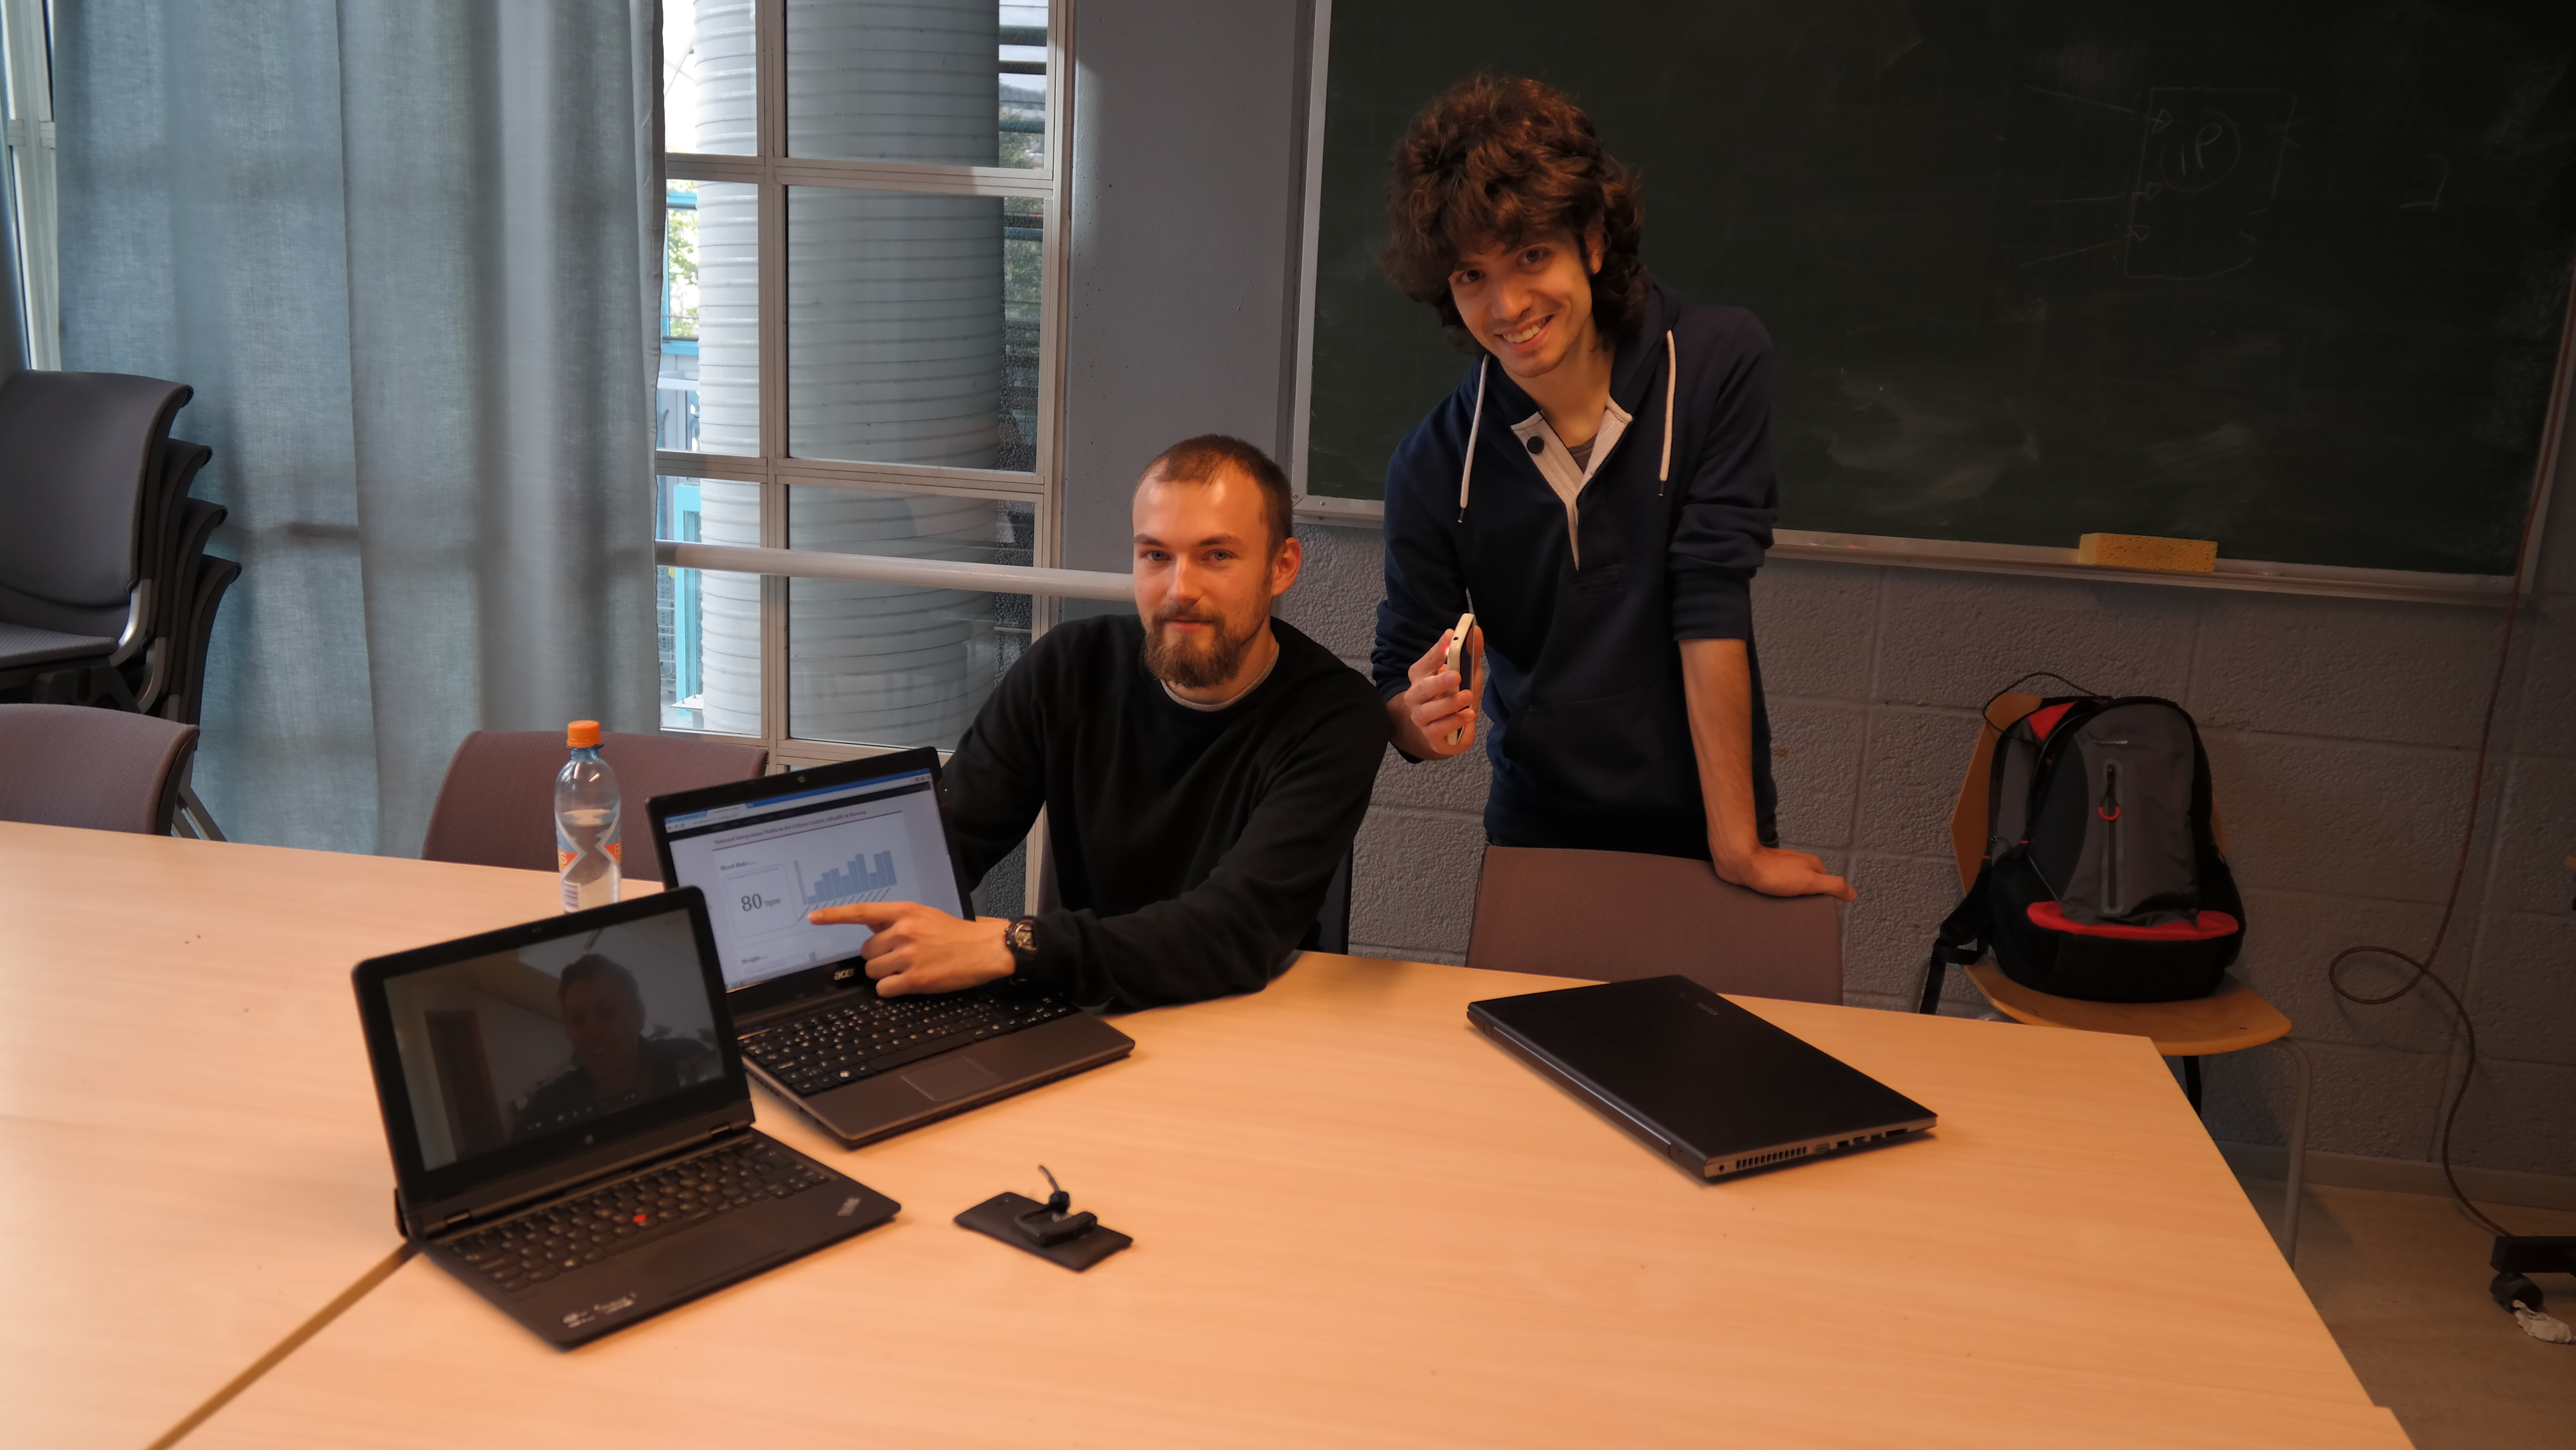
\includegraphics[scale=0.33]{../Figures/demo-m1.jpg}
\caption{Team demonstrating the product}
\label{figure:demonstration-m1}
\end{figure}

Figure \ref{figure:demonstration-m1} shows the team demonstrating the product to the customer (who took the picture).
Emanuele is holding his mobile phone running the heart rate application while Sebastian is pointing at the frontend
showing how the data is being acquired. Anders is participanting to the conversation through Skype.



%Due to timing issues we didn't manage to produce all the documentation we planned to.
%In particular we were missing the table of contents of the report and 